 \documentclass[9pt, aspectratio=169]{beamer}

%~~~~~~~~~~~~~~~~~~~~~~~~~~~~~~~~~~~~~~~~~~~~~~~~~~~~~~~~~~~~~~~~~~~~~~~~~~~~~~
% Use roboto Font (recommended)
\usepackage[sfdefault]{GoSans}
\usepackage[utf8]{inputenc}
\usepackage[T1]{fontenc}
\usepackage{makecell}
\usepackage{longtable}
%~~~~~~~~~~~~~~~~~~~~~~~~~~~~~~~~~~~~~~~~~~~~~~~~~~~~~~~~~~~~~~~~~~~~~~~~~~~~~~

%~~~~~~~~~~~~~~~~~~~~~~~~~~~~~~~~~~~~~~~~~~~~~~~~~~~~~~~~~~~~~~~~~~~~~~~~~~~~~~
% Define where theme files are located. ('/styles')
\usepackage{styles/fluxmacros}
\usefolder{styles}
% Use Flux theme v0.1 beta
% Available style: asphalt, blue, red, green, gray 
\usetheme[style=asphalt]{flux}
%~~~~~~~~~~~~~~~~~~~~~~~~~~~~~~~~~~~~~~~~~~~~~~~~~~~~~~~~~~~~~~~~~~~~~~~~~~~~~~

%~~~~~~~~~~~~~~~~~~~~~~~~~~~~~~~~~~~~~~~~~~~~~~~~~~~~~~~~~~~~~~~~~~~~~~~~~~~~~~
% Extra packages for the demo:
\usepackage{booktabs}
\usepackage{colortbl}
\usepackage{ragged2e}
\usepackage{schemabloc}
\usetikzlibrary{positioning,calc}
\usetikzlibrary{backgrounds,fit}
\usepackage{color}
% \usepackage{tikz}
\usepackage{float}
% \usetikzlibrary{positioning}
\usepackage{centernot}
% \usetikzlibrary{trees}
% \usetikzlibrary{arrows,automata}

\usepackage{amsmath}
\usepackage{natbib}
\usepackage[tableposition=top]{caption}
\usepackage{subcaption}
\bibliographystyle{abbrv}
%\setcitestyle{authoryear, open={(},close={)}}
\usepackage{threeparttable}
\usepackage{makecell}
\usepackage{pgf,tikz}
\usetikzlibrary{arrows, automata}
\usetikzlibrary{shapes.geometric}
\usetikzlibrary{positioning,calc, decorations.pathreplacing}
\usepackage{pgfplots} 

\usepackage{bbding}
\DeclareMathOperator{\E}{\operatorname{E}}
\newcommand*\circled[1]{\tikz[baseline=(char.base)]{
            \node[shape=circle,draw,inner sep=2pt] (char) {#1};}}
%~~~~~~~~~~~~~~~~~~~~~~~~~~~~~~~~~~~~~~~~~~~~~~~~~~~~~~~~~~~~~~~~~~~~~~~~~~~~~~

%~~~~~~~~~~~~~~~~~~~~~~~~~~~~~~~~~~~~~~~~~~~~~~~~~~~~~~~~~~~~~~~~~~~~~~~~~~~~~~
% Informations
\title{\shortstack{A joint model of within-host viral kinetics\\ for SARS-CoV-2 infection}}
\subtitle{Combining multiple measures of infectiousness}
\author{ }
\institute{
  Department of Epidemiology \\
  \\
  \usebeamerfont{author}\color{Gray}Harvard School of Public Health
}

\date{\today}
\titlegraphic{assets/HSPH_CCDD-logo-KO.png}
%~~~~~~~~~~~~~~~~~~~~~~~~~~~~~~~~~~~~~~~~~~~~~~~~~~~~~~~~~~~~~~~~~~~~~~~~~~~~~~

\tikzset{
  sectioner/.style={
    draw=none,
    rectangle,
    outer xsep=-0.1mm,
    minimum height=\paperheight,
    minimum width=\paperwidth,
    fill=primary
  }
}

\AtBeginSection[]{
  \begin{frame}[plain]
  \begin{tikzpicture}[remember picture,overlay]
    		\hspace*{-1pt}\node[anchor=west, sectioner] at (current page.west){};
    		% \node[anchor=south east, sectioner, fill=primary, minimum width=0.3\paperheight] at (current page.south east){};
			\node[align=center] at (current page.center){
				\usebeamerfont{title}\color{primaryLight!10}\insertsectionhead\\[0.3cm]
				% \usebeamerfont{subtitle}\color{Gray!90!black}\insertsubtitle\\[0.1cm]
				% \usebeamercolor[fg]{footer}\rule{0.7\paperwidth}{0.2pt}	\\[0.35cm]
				% \usebeamerfont{author}\color{Gray}\insertauthor\\[0.5cm]
  		% 	 \usebeamerfont{institute}\color{Gray}\insertinstitute
			};
			% \node[anchor=south,outer ysep=0.75cm] at (current page.south){\small\color{Gray!90}\insertdate};
			\node[anchor=south east,icon] at (current page.south east)(logo){\includegraphics[width=0.15\paperwidth, height=0.11\paperheight, keepaspectratio]{\inserttitlegraphic}};
		\end{tikzpicture}
  \end{frame}
}

\begin{document}

% Generate title page
\titlepage

\begin{frame}{Introduction}
    \begin{itemize}
        \item During an infectious disease outbreak, providing accurate answers to policy questions about transmission requires a detailed model of the natural history of infection and infectiousness. 
        \vfill
        \item The distribution of infectiousness is also often a fundamental parameter in dynamic models for prediction and control of an outbreak.
        \vfill
        \item Unfortunately, a direct measure of infectiousness is never available and the ``closest'' measures (e.g. culturable virus) are not timely or scalable.
        \vfill
        \item Instead, we often have proxies such as results from antigen and PCR tests, possibly combined with information about an individuals immune history.
        \vfill
        \item However, work that maps these proxies on to more gold standard measures is rare. 
        \vfill
        \item In particular, previous work has modeled viral trajectories from a single measurement source, but to date no model incorporates all measures of viral load in a single unified framework.
        \vfill
    \end{itemize}
\end{frame}

\begin{frame}{Common proxies for infectiousness}
    \begin{itemize}
        \item Viral culture
        \vfill
        \begin{itemize}
            \item Pros: ``Closest'' measure of amount of active virus being shed
            \vfill
            \item Cons: Rarely done in practice.
            \vfill
        \end{itemize}
        \item PCR tests
        \vfill
        \begin{itemize}
            \item Pros: available in most healthcare settings, can map cycle threshold values to [RNA] through calibration (either done locally or by manufacturer).
            \vfill
            \item Cons: [RNA] do not equal infectious virus particularly during latter stages of infection.
            \vfill
        \end{itemize}
        \item Rapid (LFD) tests
        \vfill
        \begin{itemize}
            \item Pros: available at home or other settings, easy to self-administer.
            \vfill
            \item Cons: less accurate (although perhaps maps to infectiousness better than to PCR result), no quantitative measure of relative infectiousness (just yes/no), perhaps a lot of user error.
            \vfill
        \end{itemize}
        \textbf{\underline{Goal:} what if we could estimate the within-host relationship between the three measures so we could impute harder to obtain measures, like viral culture, from easier to obtain measures.} 
    \end{itemize}
\end{frame}

\begin{frame}{Common proxies for infectiousness}
\begin{figure}
    \centering
    \begin{minipage}[c]{0.74\textwidth}
    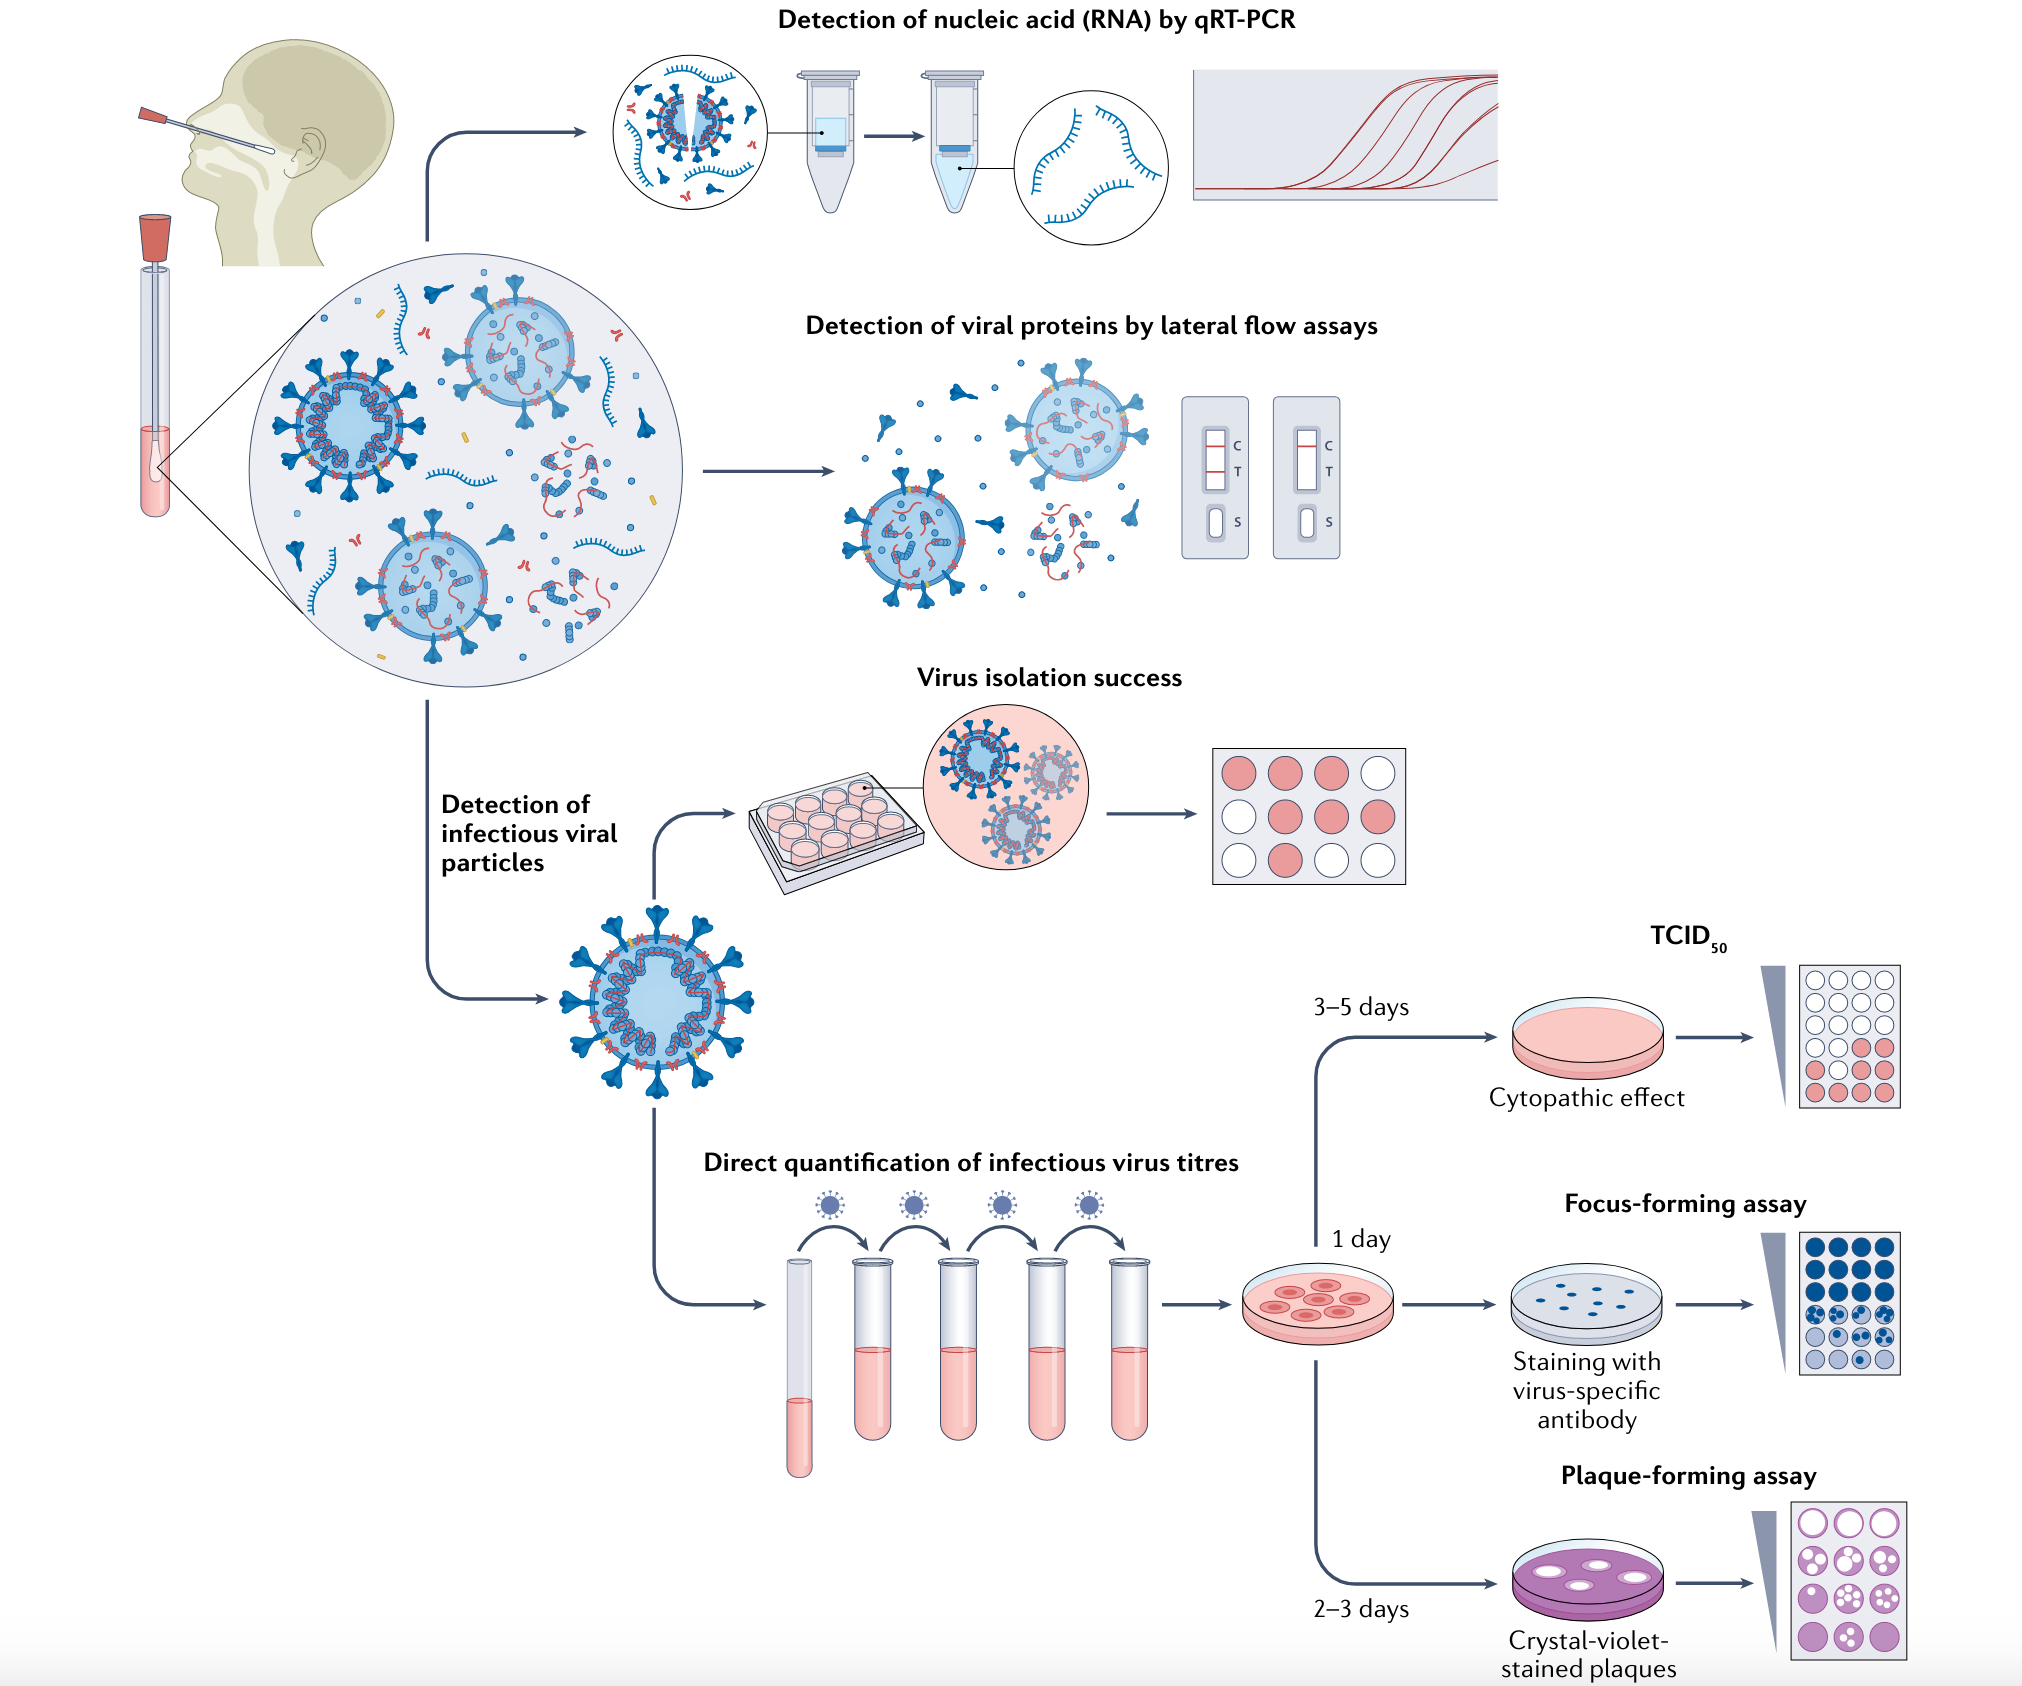
\includegraphics[width=0.80\linewidth]{Screenshot 2023-12-06 at 8.43.36 PM.png}
    \end{minipage}
    \begin{minipage}[c]{0.25\textwidth}
    \caption{Puhach, O., Meyer, B., \& Eckerle, I. (2023). SARS-CoV-2 viral load and shedding kinetics. \textit{Nature Reviews Microbiology}, 21(3).}
    \end{minipage}
    \label{fig:proxies}
\end{figure}    
\end{frame}

\begin{frame}{Data sources}
\begin{description}
    \item[\textbf{NBA:}] A prospective, longitudinal occupational cohort among NBA players and staff between March 2020 and July 2022 with 1,989 well-documented SARS-CoV-2 infections.
    \vfill
    \item[\textbf{ATACCC:}] A prospective, longitudinal, community cohort study of community contacts of newly diagnosed, PCR-confirmed SARS-CoV-2 index cases in the United Kingdom between September 2020 and May 2021 with 57 documented new infections.
    \vfill
    \item[\textbf{UIUC:}] A prospective, longitudinal, community cohort study of passively identified cases during twice-weekly screening of faculty, staff, and students at the University of Illinois Urbana Champaign between September 2020 and May 2021 with 60 documented infections.
    \vfill
    \item[\textbf{HCT:}] A prospective, longitudinal, human challenge trial of 18 unvaccinated young adults with no previous history of infection who were successfully innoculated with SARS-CoV-2. 
    \vfill
    \item[\textbf{Legacy:}] A prospective, longitudinal, human challenge trial of 18 unvaccinated young adults with no previous history of infection who were successfully innoculated with SARS-CoV-2. 
\end{description}
\end{frame}

\begin{frame}{Data sources}
\begin{table}
\centering
\small
\begin{tabular}{lcccccccccc}
\toprule
\multicolumn{1}{c}{ } & \multicolumn{2}{c}{NBA} & \multicolumn{2}{c}{ATACCC} & \multicolumn{2}{c}{UIUC} & \multicolumn{2}{c}{HCT} & \multicolumn{2}{c}{Legacy} \\
\cmidrule(l{3pt}r{3pt}){2-3} \cmidrule(l{3pt}r{3pt}){4-5} \cmidrule(l{3pt}r{3pt}){6-7} \cmidrule(l{3pt}r{3pt}){8-9} \cmidrule(l{3pt}r{3pt}){10-11}
Characteristic & N & \% & N & \% & N & \% & N & \% & N & \%\\
\midrule
Age: [0,30) & 813 & 41.0 & 0 & 0.0 & 37 & 61.7 & 0 & 0 & 67 & 42.7\\
Age: [30,50) & 873 & 44.1 & 45 & 100.0 & 17 & 28.3 & 18 & 100 & 60 & 38.2\\
Age: [50,100) & 295 & 14.9 & 0 & 0.0 & 6 & 10.0 & 0 & 0 & 30 & 19.1\\
Recurrence: No & 1790 & 90.4 & 45 & 100.0 & 60 & 100.0 & 18 & 100 & 120 & 76.4\\
Recurrence: Yes & 191 & 9.6 & 0 & 0.0 & 0 & 0.0 & 0 & 0 & 37 & 23.6\\
Variant: Pre-Alpha & 154 & 7.8 & 12 & 26.7 & 43 & 71.7 & 18 & 100 & 0 & 0.0\\
Variant: Alpha & 49 & 2.5 & 9 & 20.0 & 16 & 26.7 & 0 & 0 & 0 & 0.0\\
Variant: Delta & 187 & 9.4 & 24 & 53.3 & 0 & 0.0 & 0 & 0 & 34 & 21.7\\
Variant: Omicron & 1397 & 70.5 & 0 & 0.0 & 0 & 0.0 & 0 & 0 & 123 & 78.3\\
Variant: BA.4/BA.5 & 71 & 3.6 & 0 & 0.0 & 0 & 0.0 & 0 & 0 & 0 & 0.0\\
Variant: Other & 123 & 6.2 & 0 & 0.0 & 1 & 1.7 & 0 & 0 & 0 & 0.0\\
History: Unvaccinated & 94 & 4.7 & 45 & 100.0 & 60 & 100.0 & 18 & 100 & 0 & 0.0\\
History: Vaccinated boosted & 893 & 45.1 & 0 & 0.0 & 0 & 0.0 & 0 & 0 & 108 & 68.8\\
History: Vaccinated unboosted & 236 & 11.9 & 21 & 46.7 & 0 & 0.0 & 0 & 0 & 49 & 31.2\\
History: Vaccinated unreported & 125 & 6.3 & 0 & 0.0 & 0 & 0.0 & 0 & 0 & 0 & 0.0\\
History: Unreported & 41 & 2.1 & 0 & 0.0 & 0 & 0.0 & 0 & 0 & 0 & 0.0\\
History: Boosted unreported & 592 & 29.9 & 0 & 0.0 & 0 & 0.0 & 0 & 0 & 0 & 0.0\\
\midrule
Individuals & 1,981 &  & 45 & & 60 & & 18 & & 157 & \\
\bottomrule
\end{tabular}
\end{table}
\end{frame}

\begin{frame}{Data sources}
\begin{table}
\centering
\begin{tabular}{lccccc}
\toprule
Lab values & NBA & ATACCC & UIUC & HCT & Legacy\\
\midrule
Ct values & 21443 & 682 & 915 & 584 & 698\\
Viral cultures & 0 & 658 & 787 & 251 & 0\\
Rapid LFD tests & 0 & 641 & 789 & 252 & 0\\
Symptom diaries & 0 & 735 & 934 & 684 & 812\\
\bottomrule
\end{tabular}
\end{table}
\end{frame}

\section{Model description}
\begin{frame}{Setup}
We define the following variables:
\begin{itemize}
    \vfill
    \item $V_t$ is infectious virus  at time $t$,
    \vfill
    \item $R_t$ is viral RNA copies at time $t$,
    \vfill
    \item $Y_t$ is symptom onset (0/1) at time $t$,
    \vfill
    \item $Z_t$ is a vector of observed test or biomarker results at time $t$ including results from viral culture ($V^*_t$), RT-PCR ($R^*_t$), and lateral flow tests ($L^*_t$), e.g. $Z_t = (V^*_t, R^*_t, L^*_t)$.
    \vfill
    \item $X$ is a vector of individual covariates (e.g. sex, age, immune history),
    \vfill
    \item $S$ is a vector of test characteristics, such as swab type, gene target, etc.
    \vfill
\end{itemize}
where $t$ indexes time since inoculation and for notational convenience we suppress indexes for individuals $i$.
\vfill
\end{frame}

\begin{frame}{Goal}
    Our ultimate goal is to build a Bayesian generative model for the joint distribution
    \begin{equation*}
        f(V_t, R_t, Y_t, Z_t | X, t, S; \theta)
    \end{equation*}
    defining the within host trajectories of viral shedding and test or biomarker results over time, where $\theta$ is a vector of parameters.
    
    A natural factorization based on biology is 
    \begin{align*}
        f(&V_t, R_t, Y_t, Z_t | X, S, t; \theta) = \\ & \qquad \underbrace{f(V_t | X, t; \theta)}_{\shortstack{infectious \\ virus \\ \circled{1}}} \times \underbrace{f(R_t | V_t, X, t; \theta)}_{\shortstack{viral RNA \\ \circled{2}}} \times \underbrace{f(Y_t | V_t, R_t, X, t; \theta)}_{\shortstack{natural history \\ of symptoms \\ \circled{3}}} \times \underbrace{f(Z_t | V_t, R_t, Y_t, X, t, S; \theta)}_{\shortstack{observation \\ model \\ \circled{4}}}
    \end{align*}
    \vfill
    which is how we assume nature generates the data. 
\end{frame}


\begin{frame}{Infectious virus}
\begin{columns}
\begin{column}{0.45\textwidth}

    A common mechanistic model of an acute infection is the so-called \textit{target cell limited (TCL) model}. 
    \vfill
    \begin{align*}
    \dfrac{dT}{dt}&= -b V T \\
    \dfrac{dI}{dt}&= b V T - d I \\
    \dfrac{dV}{dt}&= p I - c V
    \end{align*}
    \vfill
    where, in its simplest form, the model includes compartments tracking the number of cells susceptible to infection ($T$), the number of productively infected cells ($I$), and the number of free virus particles ($V$).
\end{column}
\begin{column}{0.55\textwidth}
    \begin{figure}
        \centering
        \includegraphics[width=\linewidth]{tcl_example_1.pdf}
    \end{figure}
\end{column}
\end{columns}
\end{frame}

\begin{frame}{Infectious virus}
\begin{columns}
\begin{column}{0.45\textwidth}
    We instead posit a semi-mechanistic model which retains many of the features of the TCL model, but is more agnostic to the true biological structure of the response, the \textit{piece-wise exponential} model:
    \vfill
    \begin{equation*}
    \log V_t = g(t; \theta),
    \end{equation*}
    where
    \begin{equation*}
        g(t; \theta) = \begin{cases}
       \dfrac{\delta}{\omega_p} (t - (t_p - \omega_p)) & \text{if } t \leq t_p \\
        \delta - \dfrac{\delta}{\omega_r} (t - t_p) & \text{if } t > t_p,
    \end{cases}
    \end{equation*}
    \vfill
    with parameters representing peak number of infectious virus ($\delta$), proliferation time ($\omega_p$), clearance time ($\omega_r$), and time of peak ($t_p$).
\end{column}
\begin{column}{0.55\textwidth}
    \begin{figure}
    \centering
    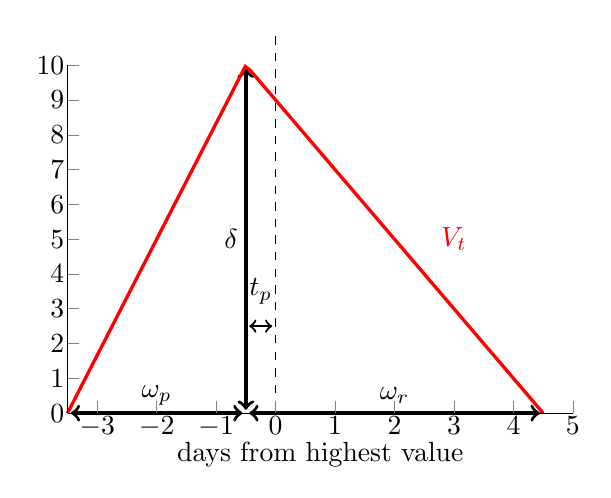
\begin{tikzpicture}
        \begin{axis}[
          no markers, domain=-3.5:4.5, samples=100,
          axis lines*=left, xlabel=days from highest value, ylabel=\empty,
          height=6cm, width=8cm,
          xtick={-5,-4,-3,-2,-1,0,1,2,3,4,5}, ytick={0,1,2,3,4,5,6,7,8,9,10},
          ymin = 0, ymax = 10, xmin =-3.5, xmax = 5,
          enlargelimits=false, clip=false, axis on top,
          grid = none, name=onset, inner sep=1pt,
          declare function={
            pefunc(\x)=(\x <= -0.5) * (10 / 3 * (\x + 3.5))  +
             (\x > -0.5) * (10 - 10 / 5 * (\x + 0.5));
            pefunc2(\x)=(\x <= 0) * (4 / 1 * (\x + 1))  +
             (\x > 0) * (4 - 4 / 2 * \x);
          }
          ]
          % \addplot [draw=none, fill=blue!20] {lnormal(1.75,0.33)}\closedcycle;
          % \addplot [very thick, blue!50!black] {lnormal(1.75,0.33)};
        %   \addplot [draw=none, fill=orange!20] {gammapdf(4, 1)}\closedcycle;
        %   \addplot [very thick, orange!50!black] {gammapdf(4, 1)};
       
          \node (a) at (axis cs: -0.5,0) { };
          \node (b) at (axis cs: 0,4) { };
          \node (c) at (axis cs: -0.5,10) { };
          \node (d) at (axis cs: -1,0) { };
          \node (e) at (axis cs: 2,0) { };
          \node (f) at (axis cs: -3.5,0) { };
          \node (g) at (axis cs: 4.5,0) { };
          \node (h) at (axis cs: 0,0) { };
          \node (i) at (axis cs: 0,11) { };
          \node (j) at (axis cs: -0.5,2.5) { };
          \node (k) at (axis cs: 0,2.5) { };
          \draw[<->, very thick](a)--(c);
          \draw[<->, very thick](a)--(f);
          \draw[<->, very thick](a)--(g);
          \draw[-, dashed](h)--(i);
          \draw[<->, thick](j)--(k);
          \node at (axis cs: 2,0.5) {$\omega_r$};
          \node at (axis cs: -2,0.5) {$\omega_p$};
          \node at (axis cs: -0.75,5) {$\delta$};
          \node at (axis cs: -0.25,3.5) {$t_p$};
          \addplot [very thick, red] {pefunc(x)};
          \node[red] at (axis cs: 3,5) {$V_t$};
        \end{axis}
    \end{tikzpicture}
    \label{fig:illustration1}
\end{figure}
\end{column}
\end{columns}
\end{frame}

\begin{frame}{viral RNA}
\begin{columns}
\begin{column}{0.45\textwidth}
    We could adapt the TCL model to track RNA by adding a compartment which tracks non-infectious virus and free floating RNA and decays at a slower rate: 
    \vfill
    \begin{align*}
    \dfrac{dT}{dt}&= -b V T \\
    \dfrac{dI}{dt}&= b V T - d I \\
    \dfrac{dV}{dt}&= p I - c V \\
    \dfrac{dR}{dt}&= q p I - e R 
    \end{align*}
    \vfill
    where $q$ the amount of viral RNA per infectious virion and $e$ is the rate of degradation and clearance of viral RNA.
\end{column}
\begin{column}{0.55\textwidth}
\begin{figure}
        \centering
        \includegraphics[width=\linewidth]{tcl_example_2.pdf}
    \end{figure}
\end{column}
\end{columns}
\end{frame}

\begin{frame}{viral RNA}
\begin{columns}
\begin{column}{0.45\textwidth}
    As before, instead we posit semi-mechanistic model:
    \vfill
    \begin{equation*}
    \log R_t = g(t; \theta^\prime),
\end{equation*}
where
\begin{equation*}
    g(t; \theta^\prime) = \begin{cases}
   \dfrac{\delta^\prime}{\omega^\prime_p} (t - (t^\prime_p - \omega^\prime_p)) & \text{if } t \leq t^\prime_p \\
    \delta^\prime - \dfrac{\delta^\prime}{\omega^\prime_r} (t - t^\prime_p) & \text{if } t > t^\prime_p,
\end{cases}
\end{equation*}
and
\begin{align*}
    \log \delta^\prime &= a_{0,\delta} + a_{1,\delta} \log \delta \\
    \log \omega^\prime_{p} &= a_{0,\omega_p} + a_{1,\omega_p} \log \omega_{p} \\
    \log \omega^\prime_{r} &= a_{0,\omega_r} + a_{1,\omega_r} \log \omega_{r} \\
    t^\prime_{p} &= a_{0, t_p} + a_{1, t_p} \cdot t_{p} 
\end{align*}
\vfill
\end{column}
\begin{column}{0.55\textwidth}
    \begin{figure}
    \centering
    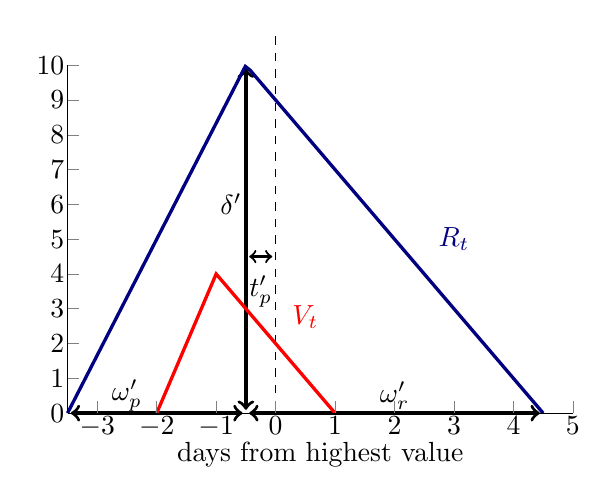
\begin{tikzpicture}
        \begin{axis}[
          no markers, domain=-3.5:4.5, samples=100,
          axis lines*=left, xlabel=days from highest value, ylabel=\empty,
          height=6cm, width=8cm,
          xtick={-5,-4,-3,-2,-1,0,1,2,3,4,5}, ytick={0,1,2,3,4,5,6,7,8,9,10},
          ymin = 0, ymax = 10, xmin =-3.5, xmax = 5,
          enlargelimits=false, clip=false, axis on top,
          grid = none, name=onset, inner sep = 1pt,
          declare function={
            pefunc(\x)=(\x <= -0.5) * (10 / 3 * (\x + 3.5))  +
             (\x > -0.5) * (10 - 10 / 5 * (\x + 0.5));
            pefunc2(\x)=(\x <= -1) * (4 / 1 * (\x + 2))  +
             (\x > -1) * (4 - 4 / 2 * (\x + 1));
          }
          ]
          % \addplot [draw=none, fill=blue!20] {lnormal(1.75,0.33)}\closedcycle;
          % \addplot [very thick, blue!50!black] {lnormal(1.75,0.33)};
        %   \addplot [draw=none, fill=orange!20] {gammapdf(4, 1)}\closedcycle;
        %   \addplot [very thick, orange!50!black] {gammapdf(4, 1)};
       
          \node (a) at (axis cs: -0.5,0) { };
          \node (a0) at (axis cs: -1,0) { };
          \node (b) at (axis cs: -1,4) { };
          \node (c) at (axis cs: -0.5,10) { };
          \node (d) at (axis cs: -2,0) { };
          \node (e) at (axis cs: 1,0) { };
          \node (f) at (axis cs: -3.5,0) { };
          \node (g) at (axis cs: 4.5,0) { };
          \node (h) at (axis cs: 0,0) { };
          \node (i) at (axis cs: 0,11) { };
          \node (j) at (axis cs: -0.5,4.5) { };
          \node (k) at (axis cs: 0,4.5) { };
          %\draw[<->, very thick](a0)--(b);
          \draw[<->, very thick](a)--(c);
          %\draw[<->, very thick](a0)--(d);
          %\draw[<->, very thick](a0)--(e);
          \draw[<->, very thick](a)--(f);
          \draw[<->, very thick](a)--(g);
           \draw[-, dashed](h)--(i);
          \draw[<->, thick](j)--(k);
          %\node at (axis cs: -0.5,0.5) {$\omega'_r$};
          \node at (axis cs: 2,0.5) {$\omega'_r$};
          %\node at (axis cs: -1.5,0.5) {$\omega'_p$};
          \node at (axis cs: -0.25,3.5) {$t'_p$};
          \node at (axis cs: -2.5,0.5) {$\omega'_p$};
          %\node at (axis cs: -1.25,2) {$\delta'$};
          \node at (axis cs: -0.75,6) {$\delta'$};
          \addplot [very thick, blue!50!black] {pefunc(x)};
          \addplot [very thick, red, domain =-2:1] {pefunc2(x)};
          \node[blue!50!black] at (axis cs: 3,5) {$R_t$};
          \node[red] at (axis cs: 0.5,2.75) {$V_t$};
        \end{axis}
    \end{tikzpicture}
    \label{fig:illustration2}
\end{figure}
\end{column}
\end{columns}
\end{frame}

\begin{frame}{Symptom onset}
     Biologically, symptoms are a manifestation of the infection or the immune response, for which the number of infectious virus and the number of viral RNA copies are at least a proxy (and one we have information about). We model symptom onset via a discrete-time hazard with a complementary log-log link:
    \begin{equation*}
        P(Y_{it} = 1 \mid Y_{i,t-1} = 0) = 1 - \exp\!\left(-\exp\!\left(\eta_0 + \eta_1 \log V_{it} + \eta_2 \log R_{it} + u_i\right)\right)
    \end{equation*}
    where $u_i \sim N(0, \sigma_u)$ captures individual heterogeneity in symptom susceptibility. The cloglog link corresponds to a discrete-time proportional hazards model; $\exp(\eta_1)$ and $\exp(\eta_2)$ are hazard ratios.
    
\end{frame}

\begin{frame}{Observation models}
For measuring infectious virus directly, there are quantitative assays based on counting plaques or focus forming units
\begin{align*}
    \log V^{*}_{t,\text{FFA}} &= \log V_t + \varepsilon_{\text{FFA}} \\
    \varepsilon_{\text{FFA}} &\sim \text{Normal}(0, \sigma_{\text{FFA}})_{lod} \\
    \log V^{*}_{t,\text{PFU}} &= \log V_t + \varepsilon_{\text{PFU}} \\
    \varepsilon_{\text{PFU}} &\sim \text{Normal}(0, \sigma_{\text{PFU}})_{lod}
\end{align*}
there are also semi-quantitative results based on the time to 50\% infection in a standard medium.
Assuming exponential viral growth in culture at rate $r$ with CPE detected at threshold $V^{\dagger}$, the latent time to detection is
\begin{equation*}
    d^{*} = a - b \log V_t + \varepsilon, \quad \varepsilon \sim \text{Normal}(0, \sigma_{\text{TCID50}})
\end{equation*}
where $b = 1/r > 0$ is the inverse culture growth rate.
Since cultures are checked daily, the observed day $D \in \{2,3,4,5,\text{neg}\}$ is interval-censored:
\begin{equation*}
    P(D = d \mid V_t) = \begin{cases}
        \Phi\!\left(\frac{2 - \mu}{\sigma}\right) & d = 2 \\
        \Phi\!\left(\frac{d - \mu}{\sigma}\right) - \Phi\!\left(\frac{d-1 - \mu}{\sigma}\right) & d \in \{3,4,5\} \\
        1 - \Phi\!\left(\frac{5 - \mu}{\sigma}\right) & d = \text{neg}
    \end{cases}
\end{equation*}
where $\mu = a - b \log V_t$ and $\sigma = \sigma_{\text{TCID50}}$.

Finally you also just have simple viral isolation
    \begin{equation*}
    V^{*}_{t,\text{culture}} \sim \text{Bernoulli}(\text{logit}^{-1}(\pi_0 + \pi_1 \log V_t)).
\end{equation*}
\end{frame}

\begin{frame}{Observation models}
Quantitative RT-PCR tests provide a cycle threshold (Ct) value, which is inversely related to the concentration of viral RNA in the clinical sample. Through calibration using an external standard with a defined number of RNA copies, the Ct value can be transformed into an estimate of the number of viral RNA copies via a characteristic curve.
$$\log R^*_t = \alpha \times (lod - C_t^*) + \kappa$$
where 
\begin{itemize}
    \item $lod$ is the limit of detection.
    \item $\alpha$ is the site-specific calibration slope.
    \item $\kappa$ is the site-specific calibration intercept.
\end{itemize}
\vfill
We model the number of viral RNA copies as a function of the Ct value via the log-normal model
\begin{align*}
    \log R^{*}_{t,\text{qPCR}} &= \log R_t + \varepsilon_{\text{qPCR}} \\
    \varepsilon_{\text{qPCR}} &\sim \text{Normal}(0, \sigma_{\text{qPCR}})_{lod}
\end{align*}
\end{frame}

\begin{frame}{Observation models}
Beyond simple measurement error of the quantitative result, a test can systematically fail due to sample quality or processing errors. We allow for false positive and false negative results by assuming that $V^{*}_{t}$ and $R^{*}_{t}$ are drawn from a mixture distribution
\vfill
\begin{align*}
    \log R^{*}_{t} & \sim \lambda_{sens} \cdot \lambda_{spec} \cdot \text{Normal}(\log R_t, \sigma_{R}) + (1 - \lambda_{sens}) \cdot \text{Exp}(1/\mu) + (1 - \lambda_{spec}) lod \\
     \log V^{*}_{t} &\sim \lambda_{sens} \cdot \lambda_{spec} \cdot \text{Normal}(\log V_t, \sigma_{V}) + (1 - \lambda_{sens}) \cdot \text{Exp}(1/\mu) + (1 - \lambda_{spec}) lod
\end{align*}
\vfill
where $\lambda_{sens}$ is the test sensitivity and $\lambda_{spec}$ is the test specificity and $\mu$ is the mean of the error distribution for false positive tests, which we set so that 90\% of distribution is within 1 Ct/PFU unit of the level of detection. We estimate $\lambda_{sens}$ and $\lambda_{spec}$ with strong priors around 95\% and 99\%.
\end{frame}

\begin{frame}{Observation models}
Lateral flow tests detect the presence of viral nucleocapsid proteins in a sample. The test is positive if the concentration of viral proteins exceeds a certain threshold. We assume the concentration of viral proteins is related to the number of infectious virus and the number of viral RNA copies, but do not directly model the true value. Instead, we model the probability of a positive antigen test as a function of the number of infectious virus particles and the number of viral RNA copies via the logistic model
\begin{equation*}
    L_t^* \sim \text{Bernoulli}(\text{logit}^{-1}(\gamma_0 + \gamma_1 \log V_t + \gamma_2 \log R_t)).
\end{equation*}
\end{frame}

\begin{frame}{Covariate effects}
    It is well established that viral shedding varies with individual characteristics such as age, variant, and prior vaccination or infection history. Therefore, we allow the parameters of the piece-wise exponential model for the number of infectious virus particles and the number of viral RNA copies, as well as the parameters of the symptom onset and observation models, to vary with individual covariates $X$. In particular, we allow the parameters of $g(t; \theta)$ and $g(t; \theta^\prime)$ to vary with $X$ via
\begin{align*}
    \delta(X) &= \delta_0 \exp(\beta_\delta X) \\
    \omega_{p}(X) &= \omega_{p_0} \exp(\beta_{\omega_p} X) \\
    \omega_{r}(X) &= \omega_{r_0} \exp(\beta_{\omega_r} X)
\end{align*}
and 
\begin{align*}
    \delta^\prime(X) &= \delta^\prime_0 \exp\{\tau_{\delta} \cdot \delta(X) + \beta^\prime_\delta X\} \\
    \omega^\prime_{p_0}(X) &= \omega^\prime_{p} \exp\{\tau_{\omega_{p}} \cdot \omega_{p}(X) + \beta^\prime_{\omega_p} X\} \\
    \omega^\prime_{r_0}(X) &= \omega^\prime_{r} \exp\{\tau_{\omega_{r}} \cdot \omega_{r}(X) + \beta^\prime_{\omega_r} X\}
\end{align*}
\end{frame}

\begin{frame}{Individual effects}
     We model residual variation in infectious virus and viral RNA at the individual level through the inclusion of individual-specific random effects for peak height, proliferation duration, clearance duration, and timing of peak, i.e. 
    \begin{align*}
        \delta_0 &= \Delta_0 \exp(\delta_{0,i}) & \delta^\prime_0 &= \Delta^\prime_0 \exp(\delta^\prime_{0,i}) \\
        \omega_{p_0} &= \Omega_{p_0} \exp( \omega_{p_0,i}) & \omega^\prime_{p_0} &= \Omega^\prime_{p_0} \exp( \omega^\prime_{p_0,i}) \\
        \omega_{r_0}  &= \Omega_{r_0} \exp(\omega_{r_0,i}) & \omega^\prime_{r_0}  &= \Omega^\prime_{r_0} \exp(\omega^\prime_{r_0,i})
    \end{align*}
    where 
    \begin{align*}
    \delta_{0,i} &\sim N(0, \sigma_{\delta_0}) & \delta^\prime_{0,i} &\sim N(0, \sigma_{\delta^\prime_0}) \\
    \omega_{p_0,i} &\sim N(0, \sigma_{\omega_{p_0}}) & \omega^\prime_{p_0,i} &\sim N(0, \sigma_{\omega^\prime_{p_0}}) \\
    \omega_{r_0,i} &\sim N(0, \sigma_{\omega_{r_0}}) & \omega^\prime_{r_0,i} &\sim N(0, \sigma_{\omega^\prime_{r_0}}).
    \end{align*}
\end{frame}

\section{Model fitting and checks}
\begin{frame}{Priors}
    \begin{figure}
        \centering
        \includegraphics[width=0.8\linewidth]{prior_pe.pdf}
    \end{figure}
\end{frame}

\begin{frame}{Priors}
    \begin{figure}
        \centering
        \includegraphics[width=0.8\linewidth]{prior_trans_pe.pdf}
    \end{figure}
\end{frame}

\begin{frame}{Priors}
    \begin{figure}
        \centering
        \includegraphics[width=0.8\linewidth]{prior_trans_times.pdf}
    \end{figure}
\end{frame}

\begin{frame}{Priors}
    \begin{figure}
        \centering
        \includegraphics[width=0.85\linewidth]{prior_trajectories.pdf}
    \end{figure}
\end{frame}

\begin{frame}{Model fitting}
    \begin{itemize}
        \item We specify weak priors on parameters based on prior literature.
        \vfill
        \item We sample from posterior distribution using MCMC.
        \vfill
        \begin{itemize}
            \item 6 chains with 3000 samples each and 1000 burn-in samples.
            \vfill
            \item Verify convergence based on standard diagnostics.
            \vfill
            \item Check observed vs. predicted fits (next slide)
        \end{itemize}
        \vfill
        \item Prior to fitting, we use simulation based approaches to sample from a known DGP to verify that our model captures true parameter value appropriately.
    \end{itemize}    
\end{frame}

\begin{frame}{Trace plots}
    \begin{figure}
        \centering
        \includegraphics[width=0.92\linewidth]{trace_plots.pdf}
    \end{figure}
\end{frame}

% \begin{frame}{Fit to ATACCC data}
%     \begin{figure}
%         \centering
%         \includegraphics[width=0.92\linewidth]{ataccc_fit.pdf}
%     \end{figure}
% \end{frame}

% \begin{frame}{Fit to UIUC data}
%     \begin{figure}
%         \centering
%         \includegraphics[width=0.92\linewidth]{ataccc_fit.pdf}
%     \end{figure}
% \end{frame}

% \begin{frame}{Fit to HCT data}
%     \begin{figure}
%         \centering
%         \includegraphics[width=0.92\linewidth]{ataccc_fit.pdf}
%     \end{figure}
% \end{frame}

% \begin{frame}{Fit and predictions in NBA data}
%     \begin{figure}
%         \centering
%         \includegraphics[width=0.92\linewidth]{nba_fit.pdf}
%     \end{figure}
% \end{frame}

% \begin{frame}{Fit and predictions in Legacy data}
%     \begin{figure}
%         \centering
%         \includegraphics[width=0.92\linewidth]{nba_fit.pdf}
%     \end{figure}
% \end{frame}


\section{Results}



% \begin{frame}{Fit and predictions in NBA data}
%     \begin{figure}
%         \centering
%         \includegraphics[width=\linewidth]{plot2.pdf}
%     \end{figure}
% \end{frame}

\begin{frame}{Results: [RNA] trajectories}
   \begin{table}[]
       \centering
       \begin{tabular}{lcc}
        \toprule
         & \multicolumn{2}{c}{Peak value} \\
        Characteristic & $\exp(\beta)$ & 95\% CrI\\
        \midrule
        Age: [30,50) & 0.99 & (0.91, 1.09)\\
        Age: [50,100) & 1.00 & (0.87, 1.13)\\
        Recurrence: Yes & 0.96 & (0.83, 1.09)\\
        Variant: Alpha & 1.04 & (0.80, 1.34)\\
        Variant: Delta & 1.20 & (0.99, 1.48)\\
        Variant: Omicron & 1.07 & (0.92, 1.26)\\
        Variant: BA.4/BA.5 & 1.14 & (0.86, 1.48)\\
        Variant: Other & 1.01 & (0.81, 1.28)\\
        History: Vaccinated boosted & 0.85 & (0.71, 1.03)\\
        History: Vaccinated unboosted & 0.87 & (0.69, 1.07)\\
        History: Vaccinated unreported & 0.82 & (0.63, 1.05)\\
        History: Unreported & 0.84 & (0.60, 1.17)\\
        History: Boosted unreported primary & 0.86 & (0.71, 1.04)\\
        \midrule
        Reference value & 16.60 & (13.99, 19.92)\\
        \bottomrule
        \end{tabular}
   \end{table}
\end{frame}

\begin{frame}{Results: [RNA] trajectories}
   \begin{table}[]
       \centering
       \begin{tabular}{lcc}
        \toprule
        & \multicolumn{2}{c}{Proliferation duration } \\
        Characteristic & $\exp(\beta)$ & 95\% CrI\\
        \midrule
        Age: [30,50) & 0.97 & (0.91, 1.04)\\
        Age: [50,100) & 1.08 & (0.99, 1.19)\\
        Recurrence & 0.86 & (0.77, 0.95)\\
        Variant: Alpha & 0.79 & (0.68, 0.91)\\
        Variant: Delta & 0.66 & (0.57, 0.75)\\
        Variant: Omicron & 0.93 & (0.82, 1.04)\\
        Variant: BA.4/BA.5 & 0.87 & (0.68, 1.14)\\
        Variant: other & 1.11 & (0.97, 1.26)\\
        History: Vaccinated boosted & 1.44 & (1.27, 1.64)\\
        History: Vaccinated unboosted & 1.17 & (1.02, 1.35)\\
        History: Vaccinated unreported & 1.22 & (1.03, 1.45)\\
        History: Unreported & 1.14 & (0.94, 1.39)\\
        History: Boosted unreported primary & 1.32 & (1.17, 1.50)\\
        \midrule
        Reference value, days & 7.29 & (6.61, 8.04)\\
        Reference value (lod), days & 4.67 & (4.23, 5.15)\\
        \bottomrule
        \end{tabular}
\   \end{table}
\end{frame}

\begin{frame}{Results: [RNA] trajectories}
   \begin{table}[]
       \centering
       \begin{tabular}{lcc}
        \toprule
        & \multicolumn{2}{c}{Clearance duration} \\
        Characteristic & $\exp(\beta)$ & 95\% CrI\\
        \midrule
        Age: [30,50) & 1.04 & (1.01, 1.08)\\
        Age: [50,100) & 1.19 & (1.13, 1.26)\\
        Recurrence & 0.74 & (0.70, 0.79)\\
        Variant: Alpha & 0.95 & (0.87, 1.04)\\
        Variant: Delta & 0.92 & (0.85, 1.00)\\
        Variant: Omicron & 0.90 & (0.84, 0.96)\\
        Variant: BA.4/BA.5 & 0.87 & (0.78, 0.97)\\
        Variant: other & 1.02 & (0.94, 1.10)\\
        History: Vaccinated boosted & 0.86 & (0.80, 0.93)\\
        History: Vaccinated unboosted & 0.74 & (0.68, 0.81)\\
        History: Vaccinated unreported & 0.79 & (0.72, 0.87)\\
        History: Unreported & 0.98 & (0.88, 1.10)\\
        History: Boosted unreported primary & 0.87 & (0.81, 0.93)\\
        \midrule
        Reference value, days & 14.55 & (13.69, 15.44)\\
        Reference value (lod), days & 9.31 & (7.96, 8.71)\\
        \bottomrule
        \end{tabular}
   \end{table}
\end{frame}

\begin{frame}{Results}
   \begin{table}[]
       \centering
       \caption{Correlation between viral and infectious virus}
       \begin{tabular}{lcccc}
        \toprule
        Parameter & $\exp(a_0)$ & 95\% CrI & $\exp(a_1)$ & 95\% CrI\\
        \midrule
        Peak ($\delta'$) & 0.85 & (0.13, 4.67) & 0.47 & (0.27, 0.64) \\
        Proliferation ($\omega_p'$) & 0.25 & (0.06, 0.77) & 0.35 & (0.22, 0.52) \\
        Clearance ($\omega_^'$) & 0.66 & (0.13, 2.32) &  0.27 & (0.17, 0.37) \\
        \midrule
        Peak time ($t_p'$) & 1.37 & (1.15, 1.64) & -0.05 & (-0.32, 0.24)\\
        \bottomrule
        \end{tabular}
       \label{tab:corr}
   \end{table}
\end{frame}


\begin{frame}{Results}
   \begin{table}[]
       \centering
       \caption{LFD positivity as a function of [RNA] and viral culture}
       \begin{tabular}{lcc}
        \toprule
        Predictor & $\exp(\gamma)$ & 95\% CrI\\
        \midrule
        log RNA copies & 1.60 & (1.41, 1.80)\\
        log PFU culturable virus & 1.27 & (1.12, 1.45)\\
        \midrule
        Intercept & -6.41 & (-7.80, -5.00)\\
        \bottomrule
        \end{tabular}
       \label{tab:lfd}
   \end{table}
\end{frame}

\begin{frame}{Possible applications}
    Example questions that could be answered:
    \begin{itemize}
        \item \textbf{For transmission modeling:} what is the distribution of infectiousness as a function of time since infection, vaccination or prior infection status, comorbidities, and other variables? 
        \vfill
        \item \textbf{For testing and screening policy recommendations:} what is the additional transmission-reduction benefit of earlier detection and isolation achievable by more rigorous policies? 
        \vfill
        \item \textbf{For isolation guidance:} what is the expected remaining infectiousness left in a person released from isolation after specific numbers of days post symptom onset, or post first positive test, with or without requirement for a negative test to leave isolation? 
    \end{itemize}

    \vfill
\end{frame}

\begin{frame}{Analysis 1: testing policy}
\begin{itemize}
    \item We could just average across posterior trajectories for each individual in our combined dataset.
    \vfill
    \item This would be relevant, for instance, for parameterizing a transmission model. 
    \vfill
    \item However, for testing and quarantine policies there's a question about the appropriate \textit{time zero}.
    \vfill
    \item In both studies cases were sampled independent of symptoms (due to contact with case in ATACCC and due to periodic testing policy in NBA data). This captured early proliferation phase which was crucial for correctly fitting our model.
    \vfill
    \item  However, in real world people often aren't aware of infection at that point. For these questions we need to condition on a meaningful event/time point to start counting from.
    \vfill
    \item In ATACCC, participants were asked to take daily rapid tests. Among cases, therefore, we can condition on first positive test and use our model to generate posterior trajectories for each individual starting from this time point and then average across trajectories.
\end{itemize}
\end{frame}

\begin{frame}{Analysis 1: testing policy}
Formally we are doing:
\begin{align*}
    \Pr[C_t > lod | t, t > T_0] &= \int_X f(C_t > lod | t, X, t > T_0)dF_X(X | t, t > T_0) \\
    \Pr[V_t > 0 | t, t > T_0] &= \int_X \int_{C_t} f(V_t | C_t)dF(C_t > lod | t, X, t > T_0)dF_X(X | t, t > T_0) \\
    \Pr[L_t = 1 | t, t > T_0] &= \int_X \int_{C_t} \int_{V_t} f(L_t | V_t, C_t) dF(V_t | C_t)dF(C_t > lod | t, X, t > T_0)dF_X(X | t, t > T_0)
\end{align*}
\end{frame}

\begin{frame}{Analysis 1: testing policy}
    \begin{figure}
        \centering
        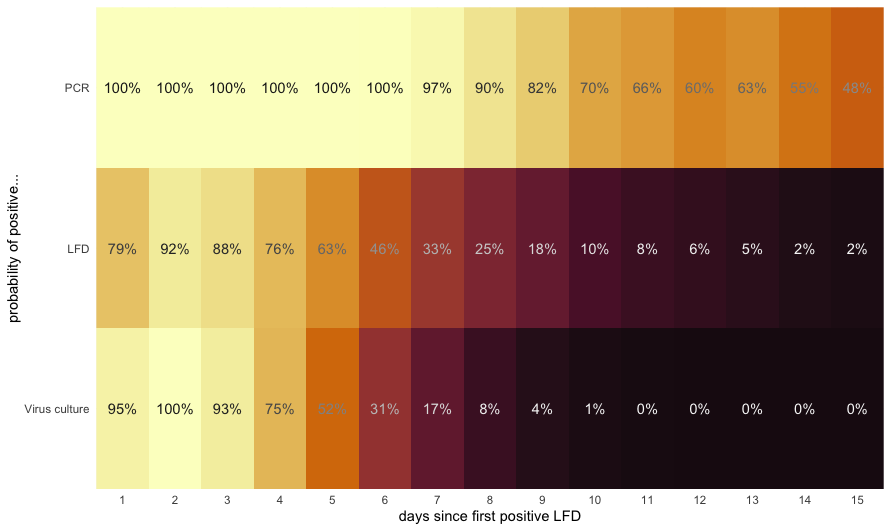
\includegraphics[width=0.8\linewidth]{probability.png}
    \end{figure}
\end{frame}

\begin{frame}{Analysis 1: testing policy}
    \begin{figure}
        \centering
        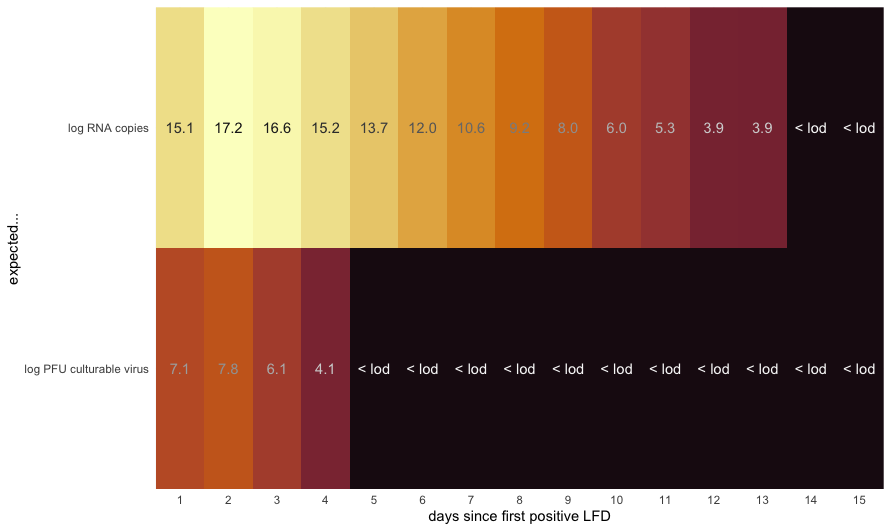
\includegraphics[width=0.8\linewidth]{expected.png}
    \end{figure}
\end{frame}

\begin{frame}{Analysis 1: testing policy}
    \begin{figure}
        \centering
        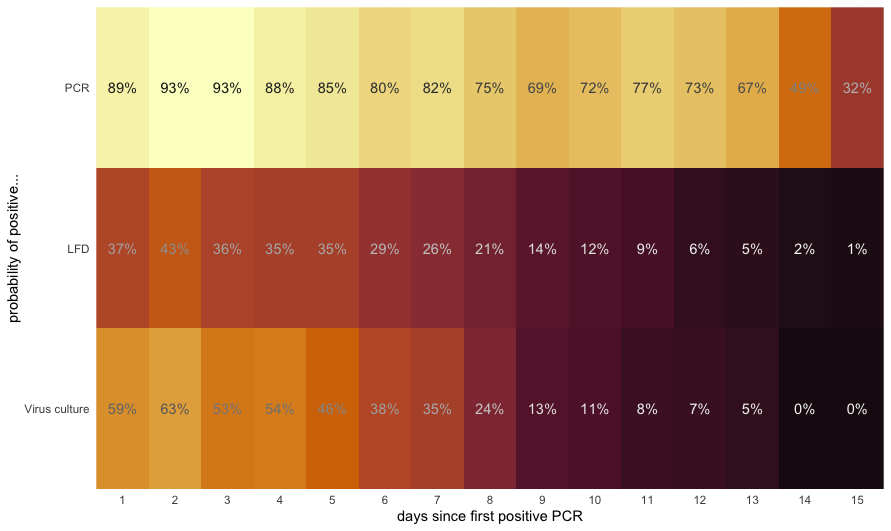
\includegraphics[width=0.8\linewidth]{probability_nba.png}
    \end{figure}
\end{frame}


\begin{frame}{Analysis 1: testing policy}
For isolation policy, we may want to know distribution of infectiousness counting from unified time zero, but conditional on whether you are LFD positive. 

By Bayes Rule:
\begin{align*}
    \Pr[V_t > 0 | L_t = 1, t, t > T_0] &= \dfrac{\Pr[L_t = 1 | V_t > 0, t, t > T_0] \Pr[V_t > 0 | t, t > T_0]}{\Pr[L_t = 1 | t, t > T_0]} 
    % &= \dfrac{\Pr(L = 1 | V > 0, t) \Pr(V > 0 | t)}{\Pr(L = 1 | V >0,  t) \Pr(V > 0 | t)  + \Pr(L = 1 | V = 0,  t) \Pr(V = 0 | t)}
\end{align*}
\end{frame}

\begin{frame}{Analysis 1: testing policy}
    \begin{figure}
        \centering
        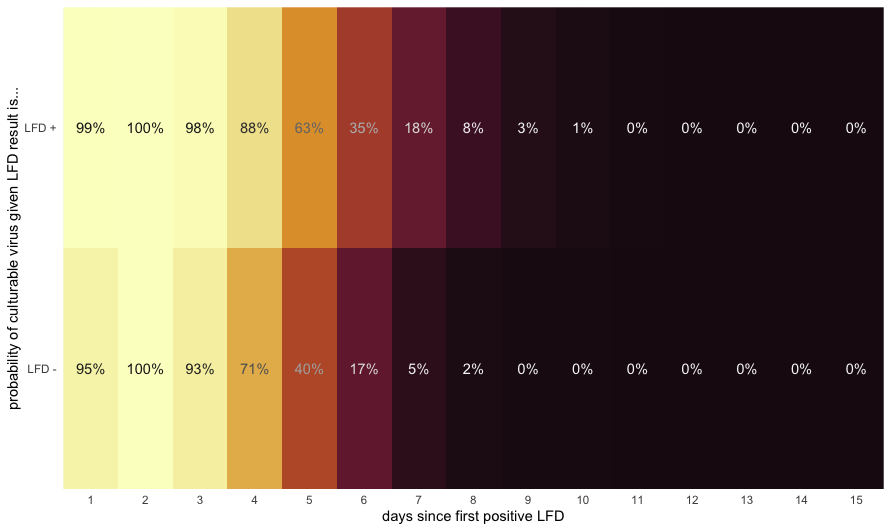
\includegraphics[width=0.8\linewidth]{probability_by_rapid_result.png}
    \end{figure}
\end{frame}

% \begin{frame}{Limitations and next steps}
%     Limitations:
%     \begin{itemize}
%         \vfill
%         \item No data on symptoms, which from an individual perspective, is probably the most relevant landmark time to count from.
%         \vfill
%         \item Heterogeneity in measurement practices across sources could create challenges.
%         \begin{itemize}
%             \item Formal test suggests they aren't different but probably under powered.
%             \vfill
%             \item Adding in site-specific parameters could allow more flexibility at cost of generalizability.
%         \end{itemize}
%         \vfill
%     \end{itemize}
%     Next steps:
%     \begin{itemize}
%         \vfill
%         \item Clean and integrate symptom data.
%         \vfill
%         \item In conversations with other groups with prospective, longitudinal data on proxies for infectiousness. 
%         \vfill
%         \item Making results more useable by other modelers and the policy community. 
%     \end{itemize}
% \end{frame}


\end{document}
